\documentclass[a4paper,fleqn]{cas-sc}

\usepackage[numbers]{natbib}
\usepackage{lipsum}
\usepackage{float}

\def\tsc#1{\csdef{#1}{\textsc{\lowercase{#1}}\xspace}}
\tsc{DP}
\tsc{LS}
\tsc{GD}

\begin{document}
\let\WriteBookmarks\relax
\def\floatpagepagefraction{1}
\def\textpagefraction{.001}
\shorttitle{}
\shortauthors{D. Papapicco et~al.}

\title [mode = title]{Likelihood estimation of an interpretable early-warning sign of critical transitions}

\author[1]{Davide Papapicco}[type=editor, orcid=0000-0001-0000-0000]
\credit{Conceptualization of this study, Methodology, Software}

\author[1]{Lauren Smith}[type=editor, orcid=0000-0001-0000-0000]
\credit{Data curation, Writing - Original draft preparation}

\author[1]{Graham Donovan}[type=editor, orcid=0000-0001-0000-0000]
\credit{Data curation, Writing - Original draft preparation}

\cormark[1]
\cortext[cor1]{Corresponding author}
\ead{g.donovan@auckland.ac.nz}

\affiliation[1]{organization={Department of Mathematics, University of Auckland},
                city={Auckland},
                country={New Zealand}}

\begin{abstract}
        This is a placeholder. \lipsum[1]
\end{abstract}

%\begin{graphicalabstract}
%\includegraphics{figs/cas-grabs.pdf}
%\end{graphicalabstract}

%\begin{highlights}
%\item Research highlights item 1
%\item Research highlights item 2
%\item Research highlights item 3
%\end{highlights}

\begin{keywords}
Early warning signals \sep 
Critical transitions \sep
Maximum likelihood estimation \sep
Stochastic dynamics \sep
\end{keywords}

\maketitle

\section{Introduction}
We will adopt a fast-slow framework to model B-tipping events.
Consider a SDE of the form

\begin{align}\label{eq:fast_slow_sde}
        dX_{t} &= f(X_{t},\mu)dt + \sigma dW_{t}\,,\\
        d\mu &= \varepsilon dt\,,
\end{align}

where $X_t$ denotes a random variable (r.v.) modelling the state of a system of interest in $\mathbb{R}^{d}$ while $\mu\in \mathbb{R}^{p}$ denotes a parameter vector.
The time evolution of the r.v. follows a deterministic drift, described by the parametrised vector field $f:\mathbb{R}^{d}\times \mathbb{R}^{p}\to \mathbb{R}^{d}$, and a stochastic diffusion of intensity $\sigma\in\mathbb{R}$, modelled by a $d-$dimensional Wiener process $W_{t}$ with zero mean and Gaussian distributed increments (i.e. $W_{s} - W_{t}\sim\mathcal{N}(0,s-t)$).
For simplicity, we will assume that the stochastic fluctuations are state-independent (i.e. ~\ref{eq:fast_slow_sde} is an additive noise SDE).
Importantly, the parameter characterising the vector field of the dynamics is not stationary but it evolves according to a slow (deterministic) linear ramp of slope $0 < \varepsilon \ll 1$.
This allows us to slowly changing the state of the system thus reflecting the multiscale time-varying forcing of real-world complex systems.
Many catastrophic collapses in ecosystems, biology and the climate systems are known to exhibit multistability in which alternative, stable equilibria coexist simultaneously.
The loss of stability or the vanishing of one of such equilibria are modelled using bifurcation normal forms.
In saddle-node (SN) B-tipping, the time changing bifurcation parameter $\mu$ eventually reaches a critical treshold $\mu=\mu_c$ at which the observed, often favorable, steady-state of the system (node) collides with an unstable equilibrium (saddle) causing annihilation of the two.
The resulting trajectory of the system (solution of ~\ref{eq:fast_slow_sde}) will tip abruptly to settle on other alternative stable equilibria which results in critical transitions with potentially catastrophic repercussions for the health of the system.

\section{Escape rate across a potential barrier}\label{sec:escape_rate}
In the following, and for the rest of this paper, we will assume that, for fixed parameters $\mu\in \mathbb{R}^{p}$ the (frozen) deterministic drift is a conservative vector field, i.e. there exist a scalar potential $V(x;\mu):\mathbb{R}^{d}\to \mathbb{R}$ such that $f(x;\mu) = -\nabla V(x;\mu)$.
Since we would like to predict B-tipping of SN type, we assume that the multistability of the system entails that $V$ is a sufficiently smooth function of the state variable and that it also grows polynomially fast as $x\to\pm\infty$.
The gradient structure of the dynamics remarkably allows to map equilibria of the vector field $f$ to critical point of its potential $V$.
In particular, globally stable equilibria of $f$ will correspond to local minima of $V$ while globally unstable equilibria are associated to local maxima of $V$.
This allows for a useful interpretation of the solution of ~\ref{eq:fast_slow_sde} as the motion of an overdamped particle governed by Langevin equation

\begin{equation}\label{eq:langevin}
        dX_{t} = -\nabla V(X_{t};\mu)dt + \sqrt{2D}dW_{t}\,,\quad D=\frac{\sigma^{2}}{2}\,.
\end{equation}

If the process is stationary (i.e. $\varepsilon\to0$) then, for a given configuration of the potential $V$ at parameter value $\mu$, the long term behaviour of a solution of the standard Langevin dynamics ~\ref{eq:langevin} is described by the random fluctuations of diffusion $\sqrt{2D}$ around local minima of $V$.

\subsection{Kramer's escape law}\label{subsec:kramer_escape_formula}
For simplicity of exposition, let us consider the $1-$dimensional case of ~\ref{eq:langevin} for which we are always guaranteed to have a potential $V$ whose gradient reconstructs the dynamics $f$.
In order to model codim$-1$ SN critical transitions, we will consider the minimum working case of a bistable system with at least one stable equilibrium for any $\mu$.
The bistability region of our system is characteriesd by subset $(\mu_1,\mu_2)\in \mathbb{R}$ of the parameter space for which two stable equilibria coexist alongside a single globally unstable equilibrium (saddle).
It follows therefore that the bistability region is bounded by two SN bifurcations at $\mu=\mu_1$ and $\mu=\mu_2$.
The resulting potential features two local minima (wells) separated by a barrier of one local maximum/saddle (hill).
Different configurations of the shape of the potential describe qualitatively different particle dynamics as represented in Figure ~\ref{fig:double_well_potential}.
Using this analogy, we will frame tipping phenomena of complex systems as saddle escapes of overdamped particles from a potential well.

\begin{figure}[t]
	      \centering
	      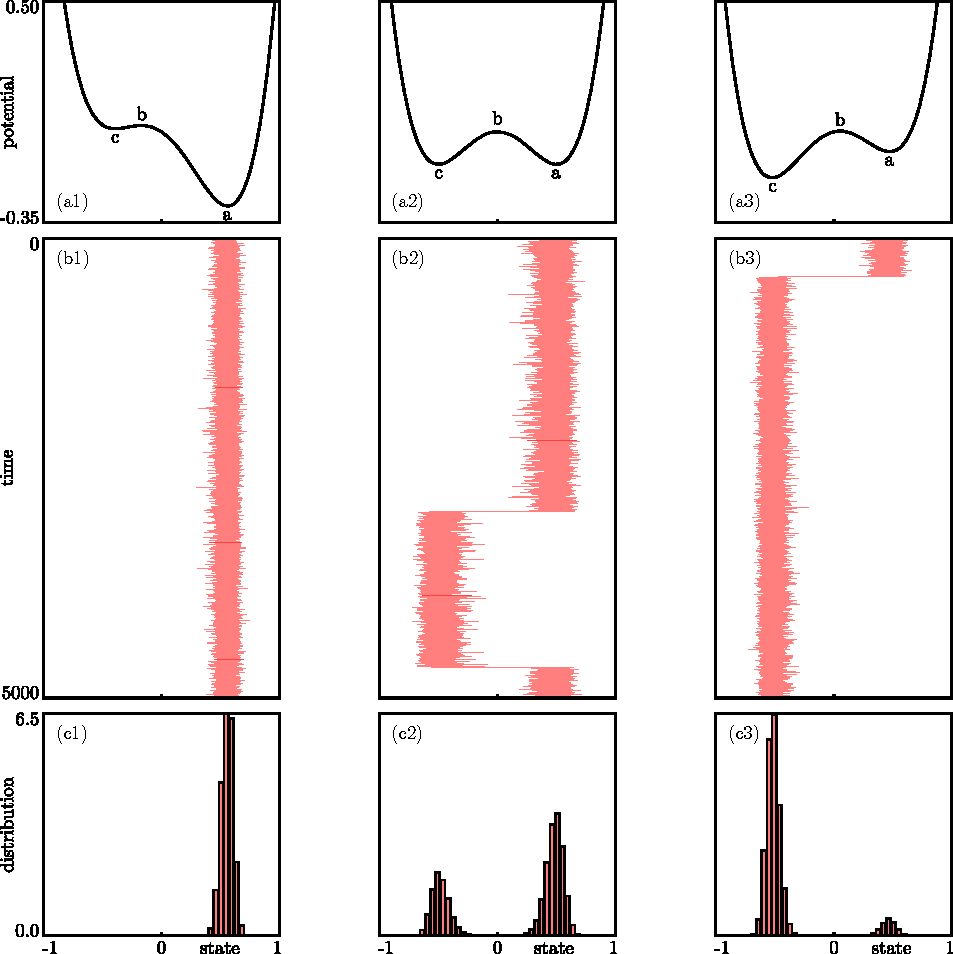
\includegraphics[keepaspectratio, width=\textwidth]{figures/double_well_potential.pdf}
        \caption{(a): only one well (global minima) exists: the particle is trapped at the bottom of this well for long times; (b) two wells are present but with different depths: the particle's motion explores the bottom of the starting well for some time before escaping over the saddle and reaching the alternative well; (c) two wells are present with equal depths: known as the Maxwell point, both wells are equiprobable and therefore the particle will equally visit the bottoms of each well for long enough time.}
        \label{fig:double_well_potential}
\end{figure}

In statistical mechanics, Kramer's formula quantifies the escape rate of particles across energy barriers when subject to Langevin's equation of motion as in ~\ref{eq:langevin}.
It is usually expressed as the reciprocal of the escape time, usually referred to as (mean) first exit time.
Different derivations of the formula based on different perspectives are available in the literature; we thus redirect the reader to [\textbf{insert citations}] for a coincise overview while in this paper we postulate its validity.
It must be noted that, while limitations on Kramer's law vailidity do exist [\textbf{cite Berglund}], our assumptions of stationary, $1-$dimensional dynamics subject to small, additive white noise fall within the applicability cases.
Given a double-well potential $V$ with desirable local minimum $x=a$ and unstable saddle equilibrium $x=b$, the rate at which particles, starting at $x=a$ and subject to white noise of intensity $\sqrt{2D}$, will escape over the saddle $x=b$ is given by

\begin{equation}\label{eq:kramer_escape_formula}
        R_{a\to b} = \frac{\sqrt{|V''(b)|V''(a)}}{2\pi}\exp\bigg(-\frac{\Delta V_{a\to b}}{D}\bigg)\,.
\end{equation}

where $\Delta V_{a\to b} = V(b) - V(a)$ quantifies the energy barrier that the Langevin overdamped particle has to overcome in order to escape and $V''$ denotes second-order differentiation of $V$ with respect to the state variable.

\subsection{An interpretable EWS}
Among the many EWS that have long been used throughout the literature, the increase in variance and autocorrelation have been the more reliable.
At the current stage however, two issues regarding the theory of generic and universal EWS still remain unanswered. The first one regards what defines the optimality of an EWS.
Suppose we have two distinct EWS that both show robustness in their trend when applied to a large enough ensemble of timeseries of the same system: how can we compare them in a systematic fashion in order to choose the better one in terms of their predictive power?
The second question concerns the interpretability of EWS.
In order for a given signal to have value as an EWS of a tipping point one has to be able to assign some sort of meaning to the computed quantity.
This is particularly important if one only has access to limited data and no ensembles of similar timeseries is available: if we compute the variance or autocorrelation from the given sample how can that single information provide us any insight on the current state of the system and, crucially, on the proximity of a B-tipping event.
It is clear that numerical values of variance and autocorrelation, if taken by themselves, do not satisfy this second criterion without a baseline to be compared to.
Until the rest of this section we argue that a modified version of Kramer's escape formula solves this issue providing interpretable values as an EWS.
Consider a generic SN bifurcation in $d-$dimensions; if the system is conservative and the noise level is small, then ~\ref{eq:kramer_escape_formula} holds well when the state of the system is far enough from the bifurcation.
Assuming the system's observed state is in a region of bistability, this entails that the two wells of the energy potential are well separated and thus the local minimum of the favorable state $x=a$ is much deeper than the local maximum of the saddle in $x=b$. 
In other words, far from the bifurcation the potential barrier $\Delta V = V(b) - V(a) \gg 0$ (we dropped the transition notation $a\to b$).
Conversely, as the SN bifurcation is approached, the stable and unstable equilibria of the system become closer and closer, resulting the in the potential barrier to reduce as the favorable well gets shallower and flatter.
This inevitably results in $\Delta V \approx 0$.
If we now consider the exponential decay of ~\ref{eq:kramer_escape_formula}, without including the curvature-depending prefactor, if immediately follows that

\begin{equation}\label{eq:escape_ews_modified}
        \exp\bigg(-\frac{\Delta V}{D}\bigg) \approx 
   \begin{cases}
       0\,, \quad \Delta V \gg 0\,,\\
       1\,, \quad \Delta V \approx 0\,. 
   \end{cases}
\end{equation}

Because we assumed the Brownian motion to be state-independent (i.e. $D\in \mathbb{R}$ does not depend on $x$), we can drop it from ~\ref{eq:escape_ews_modified} to obtain our candidate indicator $\exp(-\Delta V)$.
By denoting $\mu=\mu_{c}$ to be the parameter value at which the a SN bifurctaion involves our favorable state $x=a$ and the unstable saddle $x=b$, we finally write

\begin{equation}\label{eq:escape_ews}
        \exp(-\Delta V) \approx 
   \begin{cases}
       0\,, \quad |\mu - \mu_{c}| \gg 0\,,\\
       1\,, \quad \mu \to \mu_{c}\,. 
   \end{cases}
\end{equation}

Notice how the boundedness of ~\ref{eq:escape_ews} in $(0,1]$ conveniently solves the second issue outlined above regarding the interpretability of EWS.
As opposed to variance and autocorrelation, a numerical value of the modified escape formula provides direct interpretation of the likelihood of a B-tipping event to manifest in the near future.
If a system is far from a dangerous SN bifurcation, then the exponential decay of the potential barrier will be close to $0$; conversely, a state that is approaching a SN bifurcation would flatten the potential well and thus have resulting values of exponential decay of the potential barrier close to $1$.
In Figure ~\ref{fig:escape_ews} we depict such result for a bistable model of biomass collapse under increased harvesting.

\begin{figure}[t]
	      \centering
	      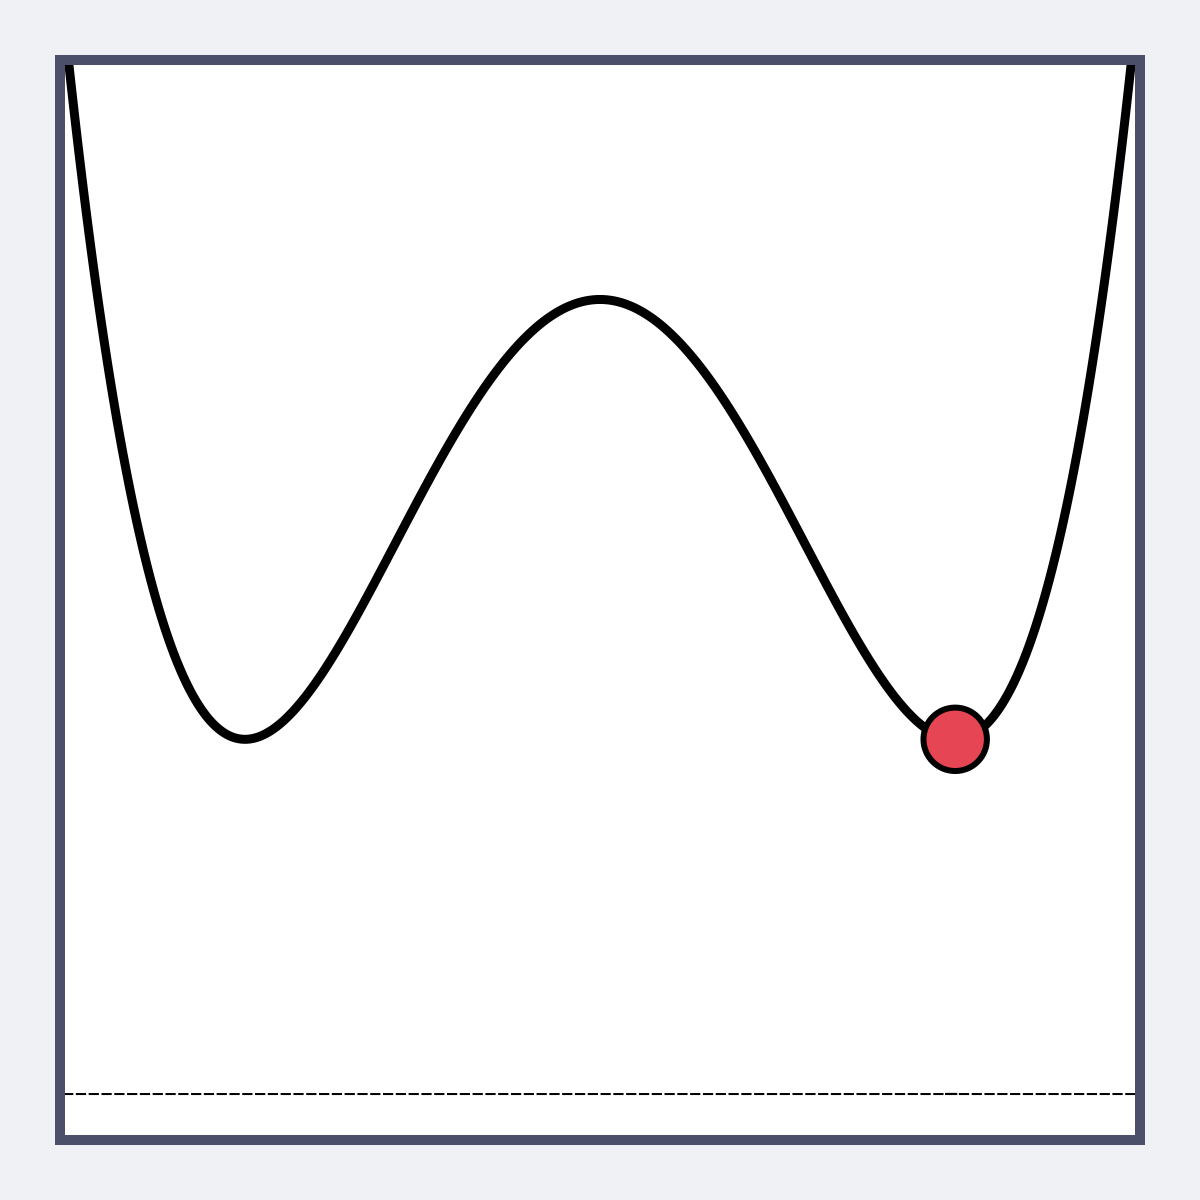
\includegraphics[keepaspectratio, width=.3\textwidth]{figures/double_well_potential.png}
        \caption{(Top): bifurcation diagram of a model of ecosystem collapse with the state $x$ (biomass) degrading as the forcing parameter $\mu$ (harvesting rate) is increased \cite{May1977}; branches of stable equilibria ($x=a$ and $x=c$) are in blue, the unstable branch ($x=b$) is in red and the vertical black thin lines indicate slices of the state of the system at different parameter values. The bistability, bounded by two SN bifurcations, is shaded in gray.
        (Middle) Configurations of the potential $V(x;\mu) = $ of the system at different parameter values (slices of the bifurcation diagram). 
        (Bottom) Modified escape EWS ~\ref{eq:escape_ews} computed out of the potential $V(x;\mu)$ between stable state $x=a$ and saddle $x=b$ within the bistability region.}
        \label{fig:double_well_potential}
\end{figure}

Finally we notice that by restricting ourselves to regions of the parameter space such that the potential barrier $\Delta V$ has range $[0,+\infty)$, the proposed EWS defines a probability measure.
This yields yet a more powerful interpretation of what discussed so far as values of ~\ref{eq:escape_ews} can be translated in likelihoods of a B-tipping event.

\section{Maximum likelihood estimation of the potential}\label{sec:mle}
The popularity of canonical EWS in the literature is in part due to their simplicity in calculating them from available data.
The increase in variance and autocorrelation in fact can be readily extracted from the timeseries of a single realisation of ~\ref{eq:langevin}.
In order for our proposed, interpretable EWS to applicable in the real-world we must be able to compute it from the solution data alone, without relying on prior knowledge of the system that generates it.
Here we describe one way to achieve this using established techniques in statistical inference. 
Suppose our sample $\{X_{n}\}_{n=0,1,\dots,N}$ is made of $N+1$ observations of the stationary state ~\ref{eq:langevin} from time $t=0$ to time $t=T$.
Suppose also that each observation is sampled at homogeneous frequency of time intervals $\Delta t = T/N$.
We can then approximate the entire sample path, beside the initial condition $X_{0}$, using Euler-Maruyama.
This defines an iterated, stochatic map of the form

\begin{equation}\label{eq:euler_maruyama}
        X_{n+1} = X_{n} -V'(X_{n};\theta)\Delta t + \sqrt{2D\Delta t}\,\xi\,,\quad \xi\sim\mathcal{N}(0,1)\,,
\end{equation}

where $V'$ denotes the first derivative (gradient) of the potential with respect to the state variable and $\theta\in\mathbb{R}^{p}$ is a vector of coefficients parameterising the potential.
We rearrange ~\ref{eq:euler_maruyama} to define the first-order time increments

\begin{equation}\label{eq:increments}
        Y_{n} := \frac{X_{n+1} - X_{n}}{\Delta t} = -V'(X_{n};\theta) + \sqrt{\frac{2D}{\Delta t}}\,\xi = -V'(X_{n};\theta) + \epsilon\,,\quad\epsilon\sim\mathcal{N}\bigg(0,\frac{2D}{\Delta t}\bigg)\,.
\end{equation}

Notice now how ~\ref{eq:increments} defines a regression to a model $V'$ of some data $\{X_{n}\}$ given a set of $N$ observations $\{Y_{n}\}$ perturbed by some Gaussian noise $\epsilon$.
This sets-up a parameter estimation problem in which one wishes to find an optimal parametrisation $\theta^*$ of the potential s.t. the residual between the model predictions $V'(X_{n};\theta^*)$ and the observations $Y_{n}$ is minimised in some sense.

\section{Applications}\label{sec:applications}

\section{Discussion}\label{sec:discussion}

\appendix
\section{Appendix}

\printcredits

\section*{Declaration of competing interest}
The authors declare that they have no known competing financial interests or personal relationships that could have appeared to influence the work reported in this paper.

\section*{Data availability}
The code used to generate the figures is available at the repository \url{https://github.com/papadeiv/papers/tree/master/2026_phys_a}.

\section*{Acknowledgements}
This wark was supported by the Royal Society of New Zealand, Te Ap\={a}rangi, Marsden funds n.XXX-XXX and n.YYY-YYY.

% Bibliography
\bibliographystyle{cas-model2-names}
\bibliography{references}

\end{document}
